\documentclass[10pt]{beamer}

\usetheme{metropolis}
\usepackage{appendixnumberbeamer}
\usepackage{booktabs}
\usepackage[scale=2]{ccicons}
\usepackage{pgfplots}
\usepgfplotslibrary{dateplot}
\pgfplotsset{compat=1.18}

\usepackage{xspace}
\usepackage{graphicx}
\usepackage{tikz}
\usetikzlibrary{positioning,arrows,shapes,decorations.pathreplacing}

\newcommand{\themename}{\textbf{\textsc{metropolis}}\xspace}
\metroset{titleformat=smallcaps,numbering=fraction}

\title{Policy Conflicts and Strategies in the Policy-Making Process}
\subtitle{POSC 315: Introduction to Public Policy}
\date{\today}
\author{David P. Adams, Ph.D.}
\institute{California State University, Fullerton}

\begin{document}

\maketitle

\begin{frame}{Table of Contents}
    \setbeamertemplate{section in toc}[sections numbered]
    \tableofcontents[hideallsubsections]
    \end{itemize}
\end{frame}


\begin{frame}
    \frametitle{Objectives}
    \begin{itemize}
        \item Understand the \alert{sources} of policy conflicts.
        \item Identify the \alert{strategies} used to manage policy conflicts.
        \item Reflect on how conflict can serve as both a \alert{challenge} and an \alert{opportunity}.
        \item Develop a foundation for applying these concepts to a \alert{real-world policy issue}.
    \end{itemize}
    \end{frame}

    \section{Defining Policy Conflicts}
    
    \begin{frame}
    \frametitle{Defining Policy Conflicts}
    \begin{columns}[T,onlytextwidth]
        \column{0.5\textwidth}
        \begin{block}{Definition}
            \begin{itemize}
                \item Policy is a \alert{course of action} or \alert{inaction} chosen by public authorities to address a given problem or interrelated set of problems.
                \item Policy is a \alert{statement} by government of what it intends to do.
                \item Policy is a \alert{guide} to action.
            \end{itemize}
        \end{block}
        \column{0.5\textwidth}
        \begin{exampleblock}{Key Elements}
            \begin{itemize}
                \item \textbf{Competing Interests}: Economic growth vs. environmental conservation
                \item \textbf{Value Clashes}: Individual freedom vs. collective welfare
                \item \textbf{Limited Resources}: Budget, time, personnel 
            \end{itemize}
        \end{exampleblock}
    \end{columns}
    \end{frame}
    
    \begin{frame}
    \frametitle{Sources of Policy Conflicts}
    \begin{enumerate}
        \item Differing Stakeholder Interests:
            \begin{itemize}
                \item Example: Businesses prioritize profits; activists prioritize sustainability.
            \end{itemize}
        \item Ideological Differences:
            \begin{itemize}
                \item Example: Debates over government intervention in healthcare.
            \end{itemize}
        \item Resource Limitations:
            \begin{itemize}
                \item Budgets spark competition among agencies or programs.
            \end{itemize}
        \item Regulatory Constraints:
            \begin{itemize}
                \item Federal and state jurisdiction overlap or contradict.
            \end{itemize}
    \end{enumerate}
    \end{frame}
    
    \begin{frame}
    \frametitle{Stakeholder Interest Conflicts}
    \begin{columns}[T,onlytextwidth]
        \column{0.5\textwidth}
        \begin{block}{Environmental Policy Example}
            \begin{itemize}
                \item \textbf{Conflict}: Economic development vs. conservation.
                \item \textbf{Stakeholders}: Industry, environmental groups, local communities.
            \end{itemize}
        \end{block}
        \column{0.5\textwidth}
        \begin{block}{Social Policy Example}
            \begin{itemize}
                \item \textbf{Conflict}: Equity vs. efficiency in welfare programs.
                \item \textbf{Stakeholders}: Taxpayers, beneficiaries, policymakers.
            \end{itemize}
        \end{block}
    \end{columns}
    \end{frame}
    
    \begin{frame}
    \frametitle{Ideological Clashes in Policy}
    \begin{itemize}
        \item Examples of Ideological Conflicts:
            \begin{enumerate}
                \item \textbf{Healthcare Reform:} Individual responsibility vs. collective welfare.
                \item \textbf{Tax Policies:} Redistribution vs. growth-oriented strategies.
            \end{enumerate}
        \item \textbf{Impact:}
            \begin{itemize}
                \item Polarized debates slow policymaking processes.
            \end{itemize}
    \end{itemize}
    \end{frame}
    
    \begin{frame}
    \frametitle{Resource Limitations}
    \begin{itemize}
        \item \textbf{Definition:} Insufficient resources create competition among stakeholders.
        \item Examples:
            \begin{enumerate}
                \item \textbf{Infrastructure Funding:} Which projects get priority?
                \item \textbf{Disaster Relief Allocation:} Balancing urgency and equity.
            \end{enumerate}
        \item \textbf{Outcome:} Resource constraints often lead to incremental decisions.
    \end{itemize}
    \end{frame}
    
    \begin{frame}
    \frametitle{Regulatory Constraints}
    \begin{itemize}
        \item \textbf{Definition:} Conflicts arising from overlapping or restrictive regulations.
        \item Example:
            \begin{itemize}
                \item Federal vs. state laws on marijuana legalization.
            \end{itemize}
        \item \textbf{Impact on Policymaking:}
            \begin{itemize}
                \item Delayed implementation.
                \item Increased litigation costs.
            \end{itemize}
    \end{itemize}
    \end{frame}
    
    \section{Managing Policy Conflicts}

    \begin{frame}
    \frametitle{Managing Policy Conflicts}
    \begin{itemize}
        \item \textbf{Key Strategies:}
            \begin{enumerate}
                \item \textbf{Negotiation:} Direct discussions for compromise.
                \item \textbf{Mediation:} Third-party facilitation.
                \item \textbf{Collaboration:} Joint decision-making.
                \item \textbf{Litigation:} Resolving disputes through courts.
            \end{enumerate}
        \item \textbf{Importance:} Effective management ensures progress and stakeholder satisfaction.
    \end{itemize}
    \end{frame}
    
    \begin{frame}
    \frametitle{Negotiation as a Strategy}
    \begin{itemize}
        \item \textbf{Definition:} Direct discussions among stakeholders to reach a compromise.
        \item \textbf{Advantages:}
            \begin{itemize}
                \item Cost-effective.
                \item Builds relationships.
            \end{itemize}
        \item \textbf{Challenges:}
            \begin{itemize}
                \item Power imbalances.
                \item Requires trust and communication.
            \end{itemize}
        \item \textbf{Real-World Example:} U.S. budget negotiations between Congress and the President.
    \end{itemize}
    \end{frame}

    \begin{frame}
        \frametitle{Mediation as a Strategy}
        \begin{itemize}
            \item \textbf{Definition:} A neutral third party facilitates discussions to resolve conflicts.
            \item \textbf{Advantages:}
                \begin{itemize}
                    \item Reduces hostility between parties.
                    \item Provides structure to negotiations.
                \end{itemize}
            \item \textbf{Challenges:}
                \begin{itemize}
                    \item Success depends on the mediator's skill and authority.
                    \item May not work if parties refuse to cooperate.
                \end{itemize}
            \item \textbf{Real-World Example:} Labor disputes resolved through federal mediation.
        \end{itemize}
        
        \begin{figure}
            \centering
            \includegraphics[width=0.6\textwidth]{mediation.png}
            \caption{Mediation in Action}
        \end{figure}
        \end{frame}
        
        \begin{frame}
        \frametitle{Collaboration as a Strategy}
        \begin{itemize}
            \item \textbf{Definition:} Joint problem-solving among stakeholders to reach shared goals.
            \item \textbf{Key Elements:}
                \begin{itemize}
                    \item Trust and communication.
                    \item Shared decision-making and resource allocation.
                \end{itemize}
            \item \textbf{Challenges:}
                \begin{itemize}
                    \item High transaction costs (time and effort).
                    \item Risk of power imbalances.
                \end{itemize}
            \item \textbf{Real-World Example:} Skokomish Watershed initiative involving government, nonprofits, and local communities.
        \end{itemize}
        
        \begin{figure}
            \centering
            \includegraphics[width=0.6\textwidth]{collaboration.png}
            \caption{Collaborative Stakeholders}
        \end{figure}
        \end{frame}
        
        \begin{frame}
        \frametitle{Litigation as a Strategy}
        \begin{itemize}
            \item \textbf{Definition:} Resolving policy conflicts through the judicial system.
            \item \textbf{Advantages:}
                \begin{itemize}
                    \item Provides a definitive resolution.
                    \item Enforces legal compliance.
                \end{itemize}
            \item \textbf{Challenges:}
                \begin{itemize}
                    \item Costly and time-consuming.
                    \item May exacerbate stakeholder animosity.
                \end{itemize}
            \item \textbf{Real-World Example:} Brown v. Board of Education resolving segregation laws.
        \end{itemize}
        \end{frame}

        \section{Collaborative Approaches}
        
        \begin{frame}
        \frametitle{Case Study: Skokomish Watershed Initiative}
        \begin{itemize}
            \item \textbf{Conflict:} Competing interests over natural resource use in the watershed.
            \item \textbf{Resolution Strategy:}
                \begin{itemize}
                    \item Collaboration among federal, state, local governments, nonprofits, and the community.
                    \item Focused on trust-building, shared goals, and resource sharing.
                \end{itemize}
            \item \textbf{Outcome:} Long-term management plan balancing conservation and community needs.
            \item \example{Skokomish Watershed Action Team (SWAT)}
        \end{itemize}
        \end{frame}
        
        \begin{frame}
        \frametitle{Costs of Collaborative Approaches}
        \begin{itemize}
            \item \textbf{What are Transaction Costs?}
                \begin{itemize}
                    \item Time, resources, and effort invested in collaboration.
                \end{itemize}
            \item \textbf{Examples of Costs:}
                \begin{itemize}
                    \item Long meetings and negotiations.
                    \item Building trust and establishing frameworks.
                    \item Managing power imbalances.
                \end{itemize}
            \item \textbf{Benefits vs. Costs:}
                \begin{itemize}
                    \item While costly, collaboration often leads to more sustainable outcomes.
                \end{itemize}
        \end{itemize}
        
        \begin{figure}
            \centering
            \begin{tabular}{lcc}
                \toprule
                & Transaction Costs & Long-Term Benefits \\
                \midrule
                Collaborative Approach & High & High \\
                Traditional Approach & Low & Moderate \\
                \bottomrule
            \end{tabular}
            \caption{Balancing Costs and Benefits of Collaboration}
        \end{figure}
        \end{frame}
        
        \begin{frame}
        \frametitle{Common Challenges in Conflict Management}
        \begin{itemize}
            \item \textbf{Trust Deficit:} Lack of faith among stakeholders.
            \item \textbf{Power Imbalances:} Dominance of one stakeholder group.
            \item \textbf{Complexity of Issues:} Multi-faceted problems with no clear solution.
        \end{itemize}
        \end{frame}

        \section{Conflict as an Opportunity and Challenge}
        
        \begin{frame}
        \frametitle{Conflict as an Opportunity}
        \begin{itemize}
            \item \textbf{Innovation:} Conflicts can inspire creative solutions.
            \item \textbf{Stakeholder Buy-In:} Resolving conflicts collaboratively builds support.
            \item \textbf{Strengthened Institutions:} Navigating conflicts enhances organizational capacity.
            \item \textbf{Example:} Affordable Care Act (ACA) negotiations.
        \end{itemize}
        \end{frame}
        
        \begin{frame}
        \frametitle{Conflict: A Challenge and Opportunity}
        \begin{columns}[T,onlytextwidth]
            \column{0.5\textwidth}
            \begin{block}{Challenges}
                \begin{itemize}
                    \item Distrust, inefficiency, stalemates.
                \end{itemize}
            \end{block}
            \column{0.5\textwidth}
            \begin{block}{Opportunities}
                \begin{itemize}
                    \item Better-informed decisions, stakeholder engagement, innovation.
                \end{itemize}
            \end{block}
        \end{columns}
        \end{frame}
        
        \begin{frame}
        \frametitle{Policy Conflict in Action: ACA}
        \begin{itemize}
            \item \textbf{Conflict:}
                \begin{itemize}
                    \item Ideological divides over healthcare access and government intervention.
                \end{itemize}
            \item \textbf{Strategies Used:}
                \begin{itemize}
                    \item Negotiation and compromise.
                    \item Incremental policymaking to build consensus.
                \end{itemize}
            \item \textbf{Outcome:} Landmark legislation improving healthcare access, albeit with ongoing debates.
        \end{itemize}
        \end{frame}

        \section{Conflict Management Strategies}
        
        \begin{frame}
        \frametitle{Incrementalism as a Conflict Strategy}
        \begin{itemize}
            \item \textbf{Definition:} Small, manageable changes to address public problems.
            \item \textbf{Pros:}
                \begin{itemize}
                    \item Stability, reduced resistance.
                    \item Easier consensus-building.
                \end{itemize}
            \item \textbf{Cons:}
                \begin{itemize}
                    \item Slow progress on urgent issues.
                    \item Limited transformative potential.
                \end{itemize}
            \item \textbf{Example:} Climate change policies using gradual carbon reduction targets.
        \end{itemize}
        \end{frame}

        \begin{frame}
            \frametitle{Adaptive Management as a Strategy}
            \begin{itemize}
                \item \textbf{Definition:} A flexible, iterative approach to policymaking that allows for adjustments based on feedback and outcomes.
                \item \textbf{Key Principles:}
                    \begin{itemize}
                        \item Monitor policy outcomes.
                        \item Incorporate feedback into future decisions.
                        \item Remain flexible in addressing challenges.
                    \end{itemize}
                \item \textbf{Real-World Example:} Climate change policies adapting to new scientific findings.
            \end{itemize}
            \end{frame}
            
            
            \begin{frame}
            \frametitle{Discussing Sources of Policy Conflict}
            \begin{itemize}
                \item \textbf{Prompt:}
                    \begin{itemize}
                        \item Which source of conflict—stakeholder interests, ideological differences, resource limitations, or regulatory constraints—do you think is most common?
                        \item Why?
                    \end{itemize}
                \item \textbf{Discussion Goal:}
                    \begin{itemize}
                        \item Identify patterns and real-world examples to contextualize conflicts.
                    \end{itemize}
            \end{itemize}
            
            \end{frame}

            \section{Conflict Management Strategies}
            
            \begin{frame}
            \frametitle{Analyzing Conflict Management Strategies}
            \begin{itemize}
                \item \textbf{Prompt:}
                    \begin{itemize}
                        \item Share an example of a policy conflict and how it was managed.
                        \item Was the chosen strategy effective? Why or why not?
                    \end{itemize}
                \item \textbf{Discussion Goal:}
                    \begin{itemize}
                        \item Evaluate the effectiveness of different conflict management approaches.
                    \end{itemize}
            \end{itemize}
            \end{frame}
            
            \begin{frame}
                \frametitle{The Conflict Resolution Pyramid}
                \begin{itemize}
                    \item \textbf{Hierarchy of Approaches:}
                        \begin{enumerate}
                            \item Avoidance (low effort): Ignore minor conflicts.
                            \item Negotiation: Direct discussions for compromise.
                            \item Collaboration: Shared decision-making.
                            \item Litigation (high effort): Court-based resolution.
                        \end{enumerate}
                    \item \textbf{Key Insight:} Strategies should match the conflict's scale and importance.
                \end{itemize}
                
                   \begin{figure}
                        \centering
                        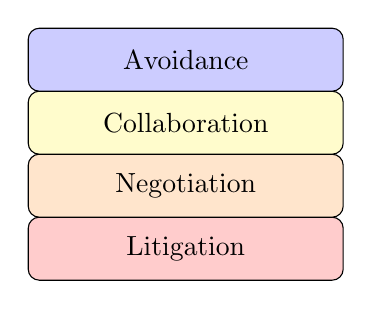
\begin{tikzpicture}[scale=0.8]
                            \draw[fill=red!20, rounded corners] (0,0) rectangle (5,1);
                            \draw[fill=orange!20, rounded corners] (0,1) rectangle (5,2);
                            \draw[fill=yellow!20, rounded corners] (0,2) rectangle (5,3);
                            \draw[fill=blue!20, rounded corners] (0,3) rectangle (5,4);
                            \node at (2.5,0.5) {Litigation};
                            \node at (2.5,1.5) {Negotiation};
                            \node at (2.5,2.5) {Collaboration};
                            \node at (2.5,3.5) {Avoidance};
                        \end{tikzpicture}
                        \caption{Conflict Resolution Pyramid}
                    \end{figure}      
                \end{frame}
            
            \begin{frame}
            \frametitle{Summary of Key Insights}
            \begin{itemize}
                \item \textbf{Conflict Sources:} Stakeholder interests, ideology, resources, regulations.
                \item \textbf{Conflict Management:} Negotiation, mediation, collaboration, litigation.
                \item \textbf{Opportunities:} Innovation, stakeholder engagement, stronger institutions.
            \end{itemize}
            \end{frame}
            
            \begin{frame}
            \frametitle{Tips for Managing Policy Conflicts}
            \begin{itemize}
                \item Develop negotiation and mediation skills.
                \item Build trust and communication among stakeholders.
                \item Focus on flexibility and adaptive strategies.
                \item Prioritize evidence-based decision-making.
            \end{itemize}
            \end{frame}

            \section{Wrapping Up}
            
            \begin{frame}
            \frametitle{Reflecting on Policy Conflict}
            \begin{itemize}
                \item How can understanding conflict improve your role as a policymaker?
                \item What strategies will you apply in your own policy work?
                \item Can conflict management turn challenges into opportunities?
            \end{itemize}
            
            \begin{figure}
                \centering
                \begin{tikzpicture}
                    \node[draw, circle, minimum size=2cm] (reflection) {\includegraphics[width=1.5cm]{reflection.png}};
                \end{tikzpicture}
                \caption{Reflecting on Policy Conflicts}
            \end{figure}
            \end{frame}
            
            \begin{frame}
            \frametitle{Discussion Questions}
            
            \begin{enumerate}
                \item How do you define policy conflict, and what are its key sources?
                \item What are the main strategies for managing policy conflicts, and how do they differ?
                \item Can conflict be both a challenge and an opportunity in the policy-making process? Why or why not?
                \item How can you apply conflict management strategies to a real-world policy issue?
            \end{enumerate}
            \end{frame}

\end{document}